\section{Sequential designs and heuristic path planning}\label{sec:heuristics}

The goal of this section is to present data collection strategies that aim at decreasing the uncertainty on the target excursion set $\es$.

\subsection{Background}
As before, let $\gp$ be a $\no$-variate random field on $\domain$. See Section \ref{sec:bg_and_notation} for a recap of the specific notation used to handle mean and covariance function of multivariate random fields.

In a sequential setting, the point of view is that $n$ data collection steps have already been performed and one wants to choose what data to collect next. After each step, the GRF model is updated using the cokriging equations \ref{eq:cokrig_mean} and \ref{eq:cokrig_cov} and we will denote by $\mathbb{P}_n$ the law of the field conditional on the data gathered up to (and including) stage $n$. More generally, we will use subscripts to denote quantities conditional on the data available up to stage $\stage$. Hence, $\mu_{\stage}(\cdot)$ and $k_{\stage}(\cdot, \cdot)$ will denote conditional mean and covariance functions conditional on the first $\stage$ data collection stages.

\begin{remark}
The type of data collected at each stage can be of any type (observation of all components of the field at a single location, observation of some components only but at several locations, ...) since the concept of \textit{generalized location} allows the cokriging equations to handle all those case by putting them on equal footage.
\end{remark}

Our goal is then to optimally select what observations to do next, where the meaning of optimal is yet to be defined. Note that here again, the concept of \textit{generalized location} allows one to consider settings where only one component of the field can be observed at each step and the strategy has to choose the spatial location as well as the component to observe (heterotopic case), or settings where several observations are allowed at each stage (batch case).

We will here restrict ourselves to the case where only one spatial location can be chosen at each stage and all components of the field are observed there (isotopic case), leaving the general case for future work.


\subsection{Optimal Sequential Design}
\label{Optdes}

\textcolor{red}{(C.T.) I suspect we need this paragraph so we cite people who have to be cited. How do we want to blend it with the rest? Personally I would get rid of this subsection.}
The mathematical expression for the optimal design involves a series
of intermixed maximizations over designs and integrals over data. In
practice, the optimal solution is intractable because of the enormous
growth over stages (see e.g. \cite{sucar2015probabilistic} and
\cite{powell2016perspectives}).  Instead, we outline heuristic
strategies.

\textcolor{red}{Here introduce the fact that candidate points are always chosen in a set $\candidates$. Mention that we usually only allow a finite set. Mention that in the specific case of robot planning, we have a waypoint graph and we thus usually take $\candidates$ to be the set of current neighbouring nodes. Mention that yes, $\candidates$ normally depends on the current location (this is for robot, in general setting, depends on the location of the last observations), but we silently suppress this dependency for readability. Nevertheless, one should always remember that the current set of candidates depends on the current setting.}
\subsection{A Naive Sampling Strategy}
\label{naive}

The simplest heuristic for adaptive sampling is to choose the next
sampling location $\spatloc_{n+1}$ based on current excursion probabilities. At stage $\stage$, one reduces the
largest levels of uncertainty by selecting the location $\spatloc_{\stage + 1}$ with
$P_{\stage}(\gp_{\spatloc_{\stage + 1}} \in T)$ closest to $0.5$..

This strategy does not account for the uncertainty in the GP
variables, \textcolor{red}{(C.T.: do we need this sentence? does it mean anything?) but is instead applicable only if one design (node) has EPs
closer to $0.5$ (see Table \ref{tab:sim_rhoab}, row
two).}

Additionally, this strategy does not account for spatial
correlation. This strategy lacks memory of where it has been and where
the uncertainty has been reduced, and therefore susceptible to local
minima.

\subsection{Myopic Path Planning}
\label{sec:myopic}

The myopic (greedy) strategy which we present here is optimal if we
imagine taking only one more stage of measurements. This selection
strategy is based on expected uncertainty reduction, but it is a
heuristic because there is no anticipation of what the subsequent
designs might offer beyond the first stage.

Based on the currently available data the myopic strategy selects the location that leads to the biggest expected reduction in IBV:
\begin{criterion}[Myopic]
\begin{equation}\label{critSEQ}
    \spatloc_{\stage + 1} = \argmin_{\spatloc \in \candidates} \EIBV_{\stage}\left(\spatloc\right)
\end{equation}
\end{criterion}

The expected IBV might be efficiently computed for each candidate points using Proposition \ref{propo2}. Once the best location has been selected, a stage of observation is performed there, the GP model is updated, yielding a conditional law $\mathbb{P}_{\stage + 1}$ and the process is repeated.

Even though this myopic strategy is non-anticipative, it still gives a
reasonable approach for creating designs in many
applications. Moreover, it can be implemented in a way that is not too demanding on computational power, making it well-suited for embedding on autonomous mobile survey platform (see Section \ref{sec:case_study} for an example).


\subsection{Look-ahead Trajectory Planning}\label{sec:LA}

We now extend the myopic strategy to a look-ahead strategy. We consider two stages of
measurements, and the strategy is then optimal in the sense that it accounts consistently for the expectations and minimizations in these two stages, but still without including any planning beyond those two steps.

\medskip

Say we have collected data up to stage $n$. The principle of two-steps lookahead
strategies is to select the next observation location $\spatloc_{\stage + 1}$ that would yield the biggest exepcted decrease in IBV if we were to (optimally) add one more observation after the one at $\spatloc_{\stage + 1}$. In order to formalize this concept, we need to be able to talk about the EIBV in the future (after observation $\stage + 1$ has been made). The definition \ref{def:eibv} of $\currentEIBV$ includes a subscript to stress that expectations are taken with respect the conditional law at stage $n$. We will extend this notion by writing $\currentEIBV(\cdot; u, y)$ to denote EIBV where expectations are taken conditional on the data available at $n$ an on an additional observation $y$ at $u$.

  \begin{criterion}[2-steps lookahead]
      The next observation location $\spatloc_{\stage + 1}$ is selected according to
      \begin{align}\label{critLA}
          \spatloc_{\stage + 1} = \argmin_{\spatloc \in \candidates}~ \mathbb{E}_{\stage}\left[\min_{\spatloc' \in
                  \candidates(\spatloc)} \EIBV_{\stage}\left(\spatloc' ; \spatloc,
      Y\right)\right]
      \end{align}
  where $Y$ is a random variable distributed according to the conditional
  law of $\gp_{\spatloc}$ at step $\stage$ (note it silently depends on the considered point
  $\spatloc$). Here, the dependence of the set of candidates on the current location has been made explicit for the second stage of measurements.
  \end{criterion}

\begin{remark}
In a practical setting, the first expectation might be computed by Monte
Carlo sampling of data $Y$ from its conditional
distribution. For each of these data samples, the second expectation
is solved using the closed-form expressions for EIBV provided by Proposition \ref{propo2}, now with conditioning on the first stage data already going into the mean and covariances in Eqs. \eqref{eq:cokrig_mean} and \eqref{eq:cokrig_cov}.
\end{remark}

\begin{remark}
All our results have been formulated in a noiseless setting. That is, to us an observation $y$ at $\spatloc$ is a realization of $\gp_{\spatloc$. Generalization to a noisy setting where $y$ is a realization of $\gp_{\spatloc} + \epsilon$ with epsilon some noise process may be performed by including noise covariance matrices where necessary.
\end{remark}

\subsection{Simulation study}
\label{sec:simulations}

\susubsection{Static and Sequential Sampling Designs}
\label{sec:sampling_designs}

%Three different designs are considered as indicated in Figure \ref{fig:stat_design}. 
%\begin{figure}[h!]
%\centering
%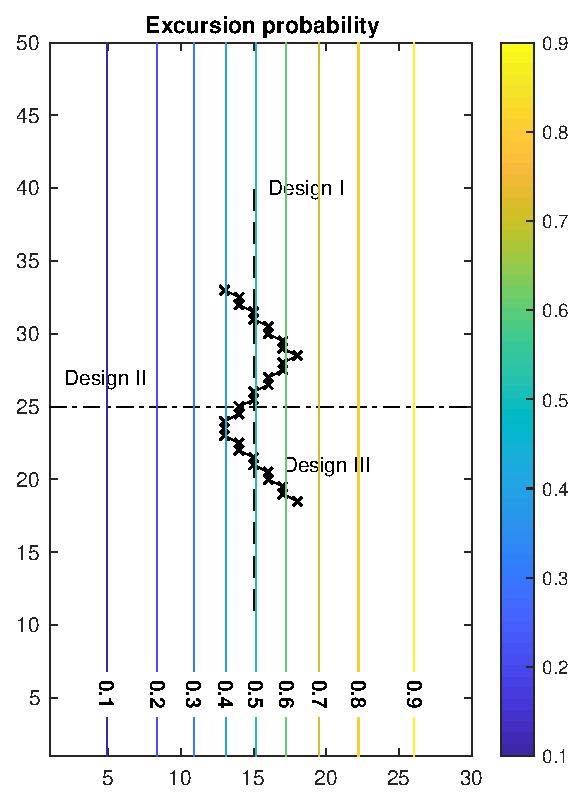
\includegraphics[width=0.65\textwidth]{Figures/Des3.eps}
%\caption{Three different static survey designs plotted on the initial EP.}\label{fig:stat_design}
%\end{figure}
%In this display the designs are plotted along with the prior probability contours of the ES for the reference parameter inputs. 

We compare three different static designs denoted
\textit{static\_north}, \textit{static\_east}, and
\textit{static\_zigzag} with the three described sequential approaches
\textit{naive}, \textit{myopic}, and \textit{look-ahead}. The static
sampling paths are pre-determined and cannot be altered and represent
the pre-planned strategies used in most current AUV operational survey
designs.

For a fixed survey length, a closed-form expression for the EIBV is
available as in Eq. \eqref{eq:eibv}. However, for the sequential
approaches this is not the case. For comparison the properties are
therefore evaluated using Monte Carlo sampling over several replicates
of realizations from the model while conducting simulated sequential
surveys for each one. Fig. \ref{fig:Eprob} shows the conditional EP,
given data gathered along the north-south survey lines in these
displays. In the Monte Carlo replicates, such results are repeatedly
computed to approximate the EIBV. We also compare predictive
performance measured by root mean square error (RMSE) for temperature
and salinity estimates as well as also the variance reduction in these
two variables. It is important to note that the objective function
used by the agent \kc{First of 'agent'. Define it or change it
  to 'robot'? Note further uses below.} is focused on reducing the
EIBV, but we nevertheless expect that we will achieve good predictive
performance for criteria such as RMSE as well. Another non-statistical
criteria that is important for practical purposes is the computational
time needed for the strategy, as this will impact the performance for
an embedded system.

%\begin{figure}[h!]
%\centering
%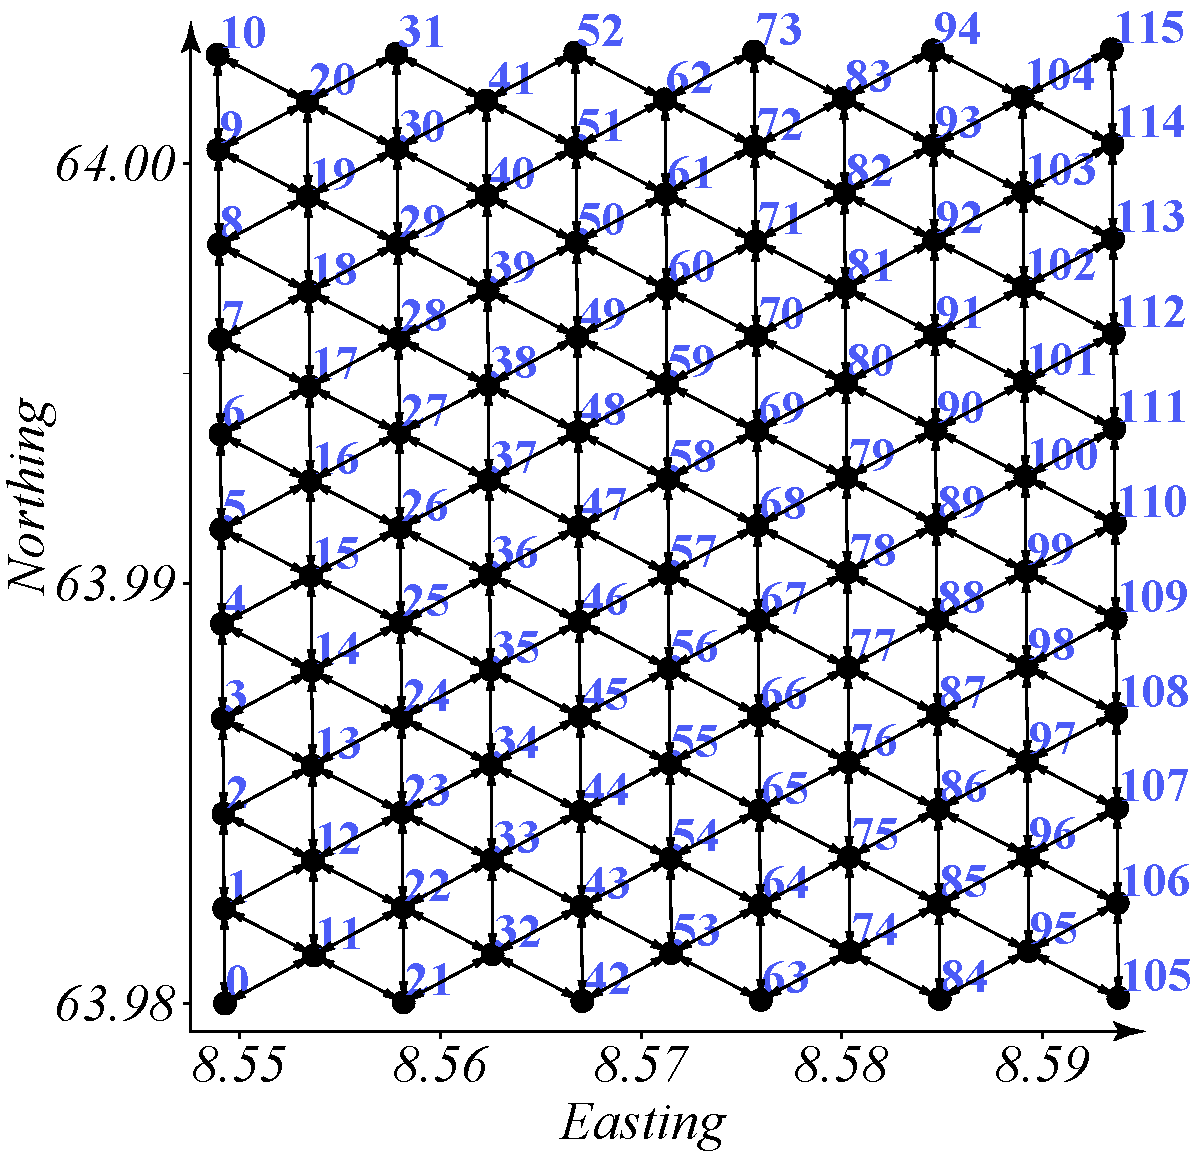
\includegraphics[width=0.50\textwidth]{Figures/sim/wp_graph_paper.pdf}
%\caption{The equilateral waypoint graph used to discretize the
%  trajectory choices over the $31\times31$ grid used to discretize the GP.}
%\label{fig:wp_graph}
%\end{figure}

\begin{figure}[!h] 
\centering 
\subfigure[The waypoint graph.]{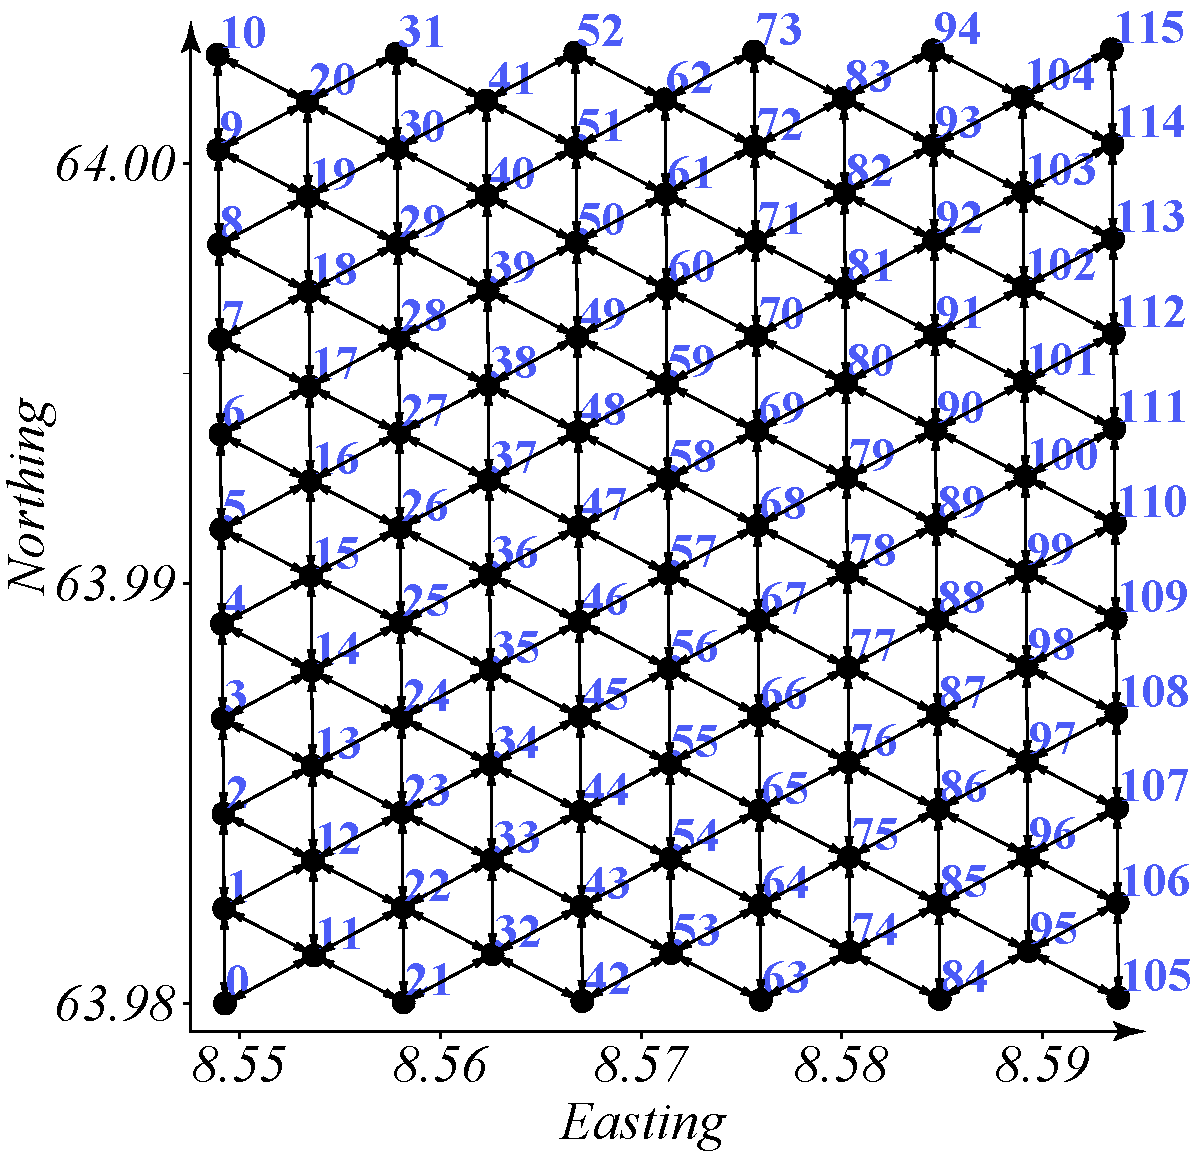
\includegraphics[width =
0.49\textwidth]{Figures/sim/wp_graph_paper.pdf}\label{fig:wp_graph_a}}
\hfill
\subfigure[The waypoint graph in 3D.]{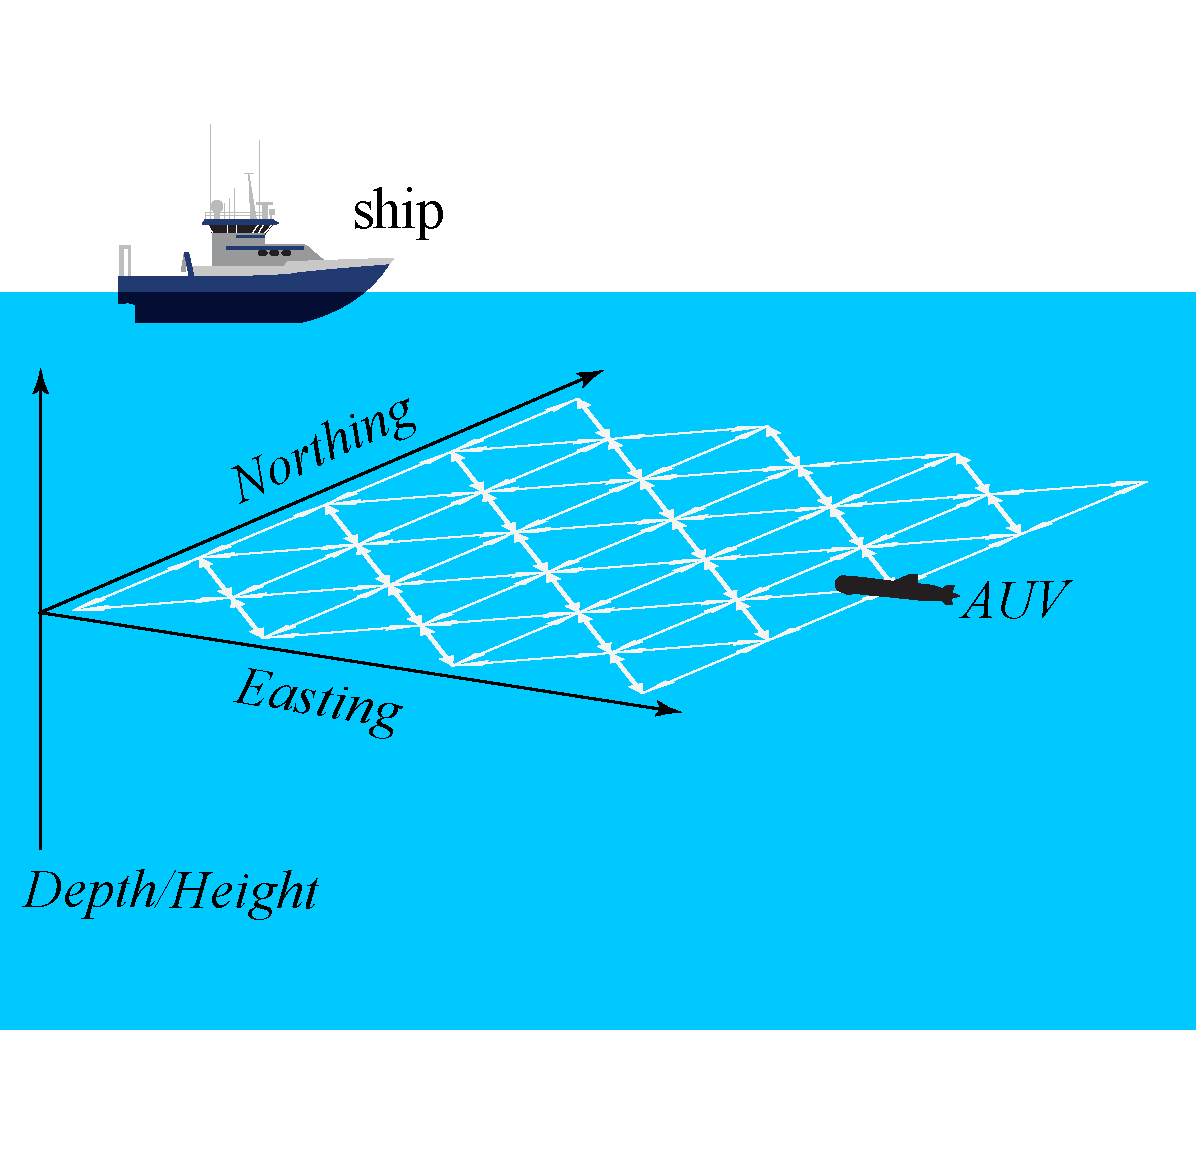
\includegraphics[width =
0.49\textwidth]{Figures/sim/wp_graph_3d.pdf}\label{fig:wp_graph_b}}
\caption{\ref{fig:wp_graph_a} The equilateral waypoint graph used to discretize the
trajectory choices over the $31\times31$ grid used to discretize the GP.
\ref{fig:wp_graph_b} The waypoint grid shown in a 3D environment.}
\label{fig:wp_graph}
\end{figure}

Each strategy is conducted on an equilateral grid as shown in
Fig. \ref{fig:wp_graph}. The sequential sampling agent starts at the
center East-West coordinate at the southern end of the domain (node 53
\kc{Maybe color this node differently and modify the caption?}). The
AUV moves along edges in the waypoint graph while the vehicle makes
measurements. The data is assimilated into the GP model before an
evaluation of the next node to sample is conducted at the end of the
edge.

\subsection{Simulation Results}

A total of 100 replicate simulations were conducted with all
strategies. The results are shown in Fig. \ref{fig:sim_results}, where
the different criteria are plotted as a function of survey
distance. Fig. \ref{fig:avg_ev} shows the resulting drop in IBV for
each of the six strategies. IBV reduction occurs most under the
\textit{myopic} and \textit{look-ahead} strategies, each performing
almost equally; this is expected as the two criteria
(Eq. \eqref{critSEQ} and \eqref{critLA}) are sensitive to differences
in IBV. The \textit{static\_north} design also does well here because
the path is parallel to the boundary between the water masses.

\begin{figure}[h!]
  \centering
  % \subfigure[Excursion set variance $E_{\by}(p[1-p])$.]{\label{fig:avg_ev}\includegraphics[height=0.49\textwidth]{Figures/sim/avg_EV.pdf}}
  \subfigure[IBV.]{\label{fig:avg_ev}\includegraphics[height=0.49\textwidth]{Figures/sim/avg_EV.pdf}}
  \hfill
  \subfigure[RMSE between estimated field and truth.]{\label{fig:avg_rmse}\includegraphics[height=0.49\textwidth]{Figures/sim/avg_RMSE.pdf}}
  \hfill 
  \subfigure[Explained variance $\bR^{2}$.]{\label{fig:avg_r2}\includegraphics[height=0.49\textwidth]{Figures/sim/avg_R2.pdf}}
  \hfill 
  \subfigure[Computational time for inferencing.\kc{I see only 
    lines associated with 4 variables showing in the graph. Where is
    static\_north and static\_east?}]{\label{fig:avg_time}\includegraphics[height=0.49\textwidth]{Figures/sim/avg_Time.pdf}} 
\caption{Simulation results from 100 replicate simulations for 10
  sampling choices/stages on the grid. \kc{Vertical lines show large
    variation in replicate results.}}  
\label{fig:sim_results}
\end{figure}

Fig. \ref{fig:avg_rmse} and \ref{fig:avg_r2} show the resulting drop
in RMSE and increase in explained variance, respectively. Both
\textit{myopic} and \textit{look-ahead} strategies perform well here,
but some of the \textit{static\_east} and \textit{static\_zigzag} also
achieve good results because they are pre-determined to cover large
parts of the domain without re-visitation. Sequential strategies
targeting IBV will sometimes not reach similar coverage, as
interesting data may draw the path into twists and turns. There is
relatively large variety in the replicate results as indicated by the
vertical lines. Nevertheless, the ordering of strategies is similar.


Fig. \ref{fig:avg_time} shows the computational effort: the
\textit{naive} strategy is on par with the static designs, while the
\textit{myopic} strategy is slower. The \textit{look-ahead} is even
slower, reaching levels that are nearly impractical for execution on a
vehicle. Some pruning of the graph is performed to improve the
performance, such as ruling out repeated visitations and
back-and-forth routes. Some of the intermediate results are also
stored for longer planning horizons. Further pruning of branches or
inclusion of other heuristics could be included for better
performance. Then again, the inclusion of heuristics is likely a
contributing factor for the \textit{look-ahead} strategy failing to
outperform the \textit{myopic} strategy.

In Fig. \ref{fig:route_choices}, the realized sampling paths for each
of the sequential schemes and static designs are shown. The
\textit{naive} strategy often gets stuck in the southern part of the
domain because it is too focused on the probabilities near $0.5$. The
\textit{myopic} strategy covers a wider domain than the naive or
look-ahead. There are several reasons for this. First, a greedy
approach will tend to put more emphasis on promising locations close
to the agent, which may lead away from the centre. Second, as the
agent evaluates the impact of locations further away (look-ahead)
where assimilated data has less predictive power, the GP model (which
is centered here) will act to restrict paths deviating from the
central zone.

We studied the sensitivity of the results by modifying the input
parameters to have different correlations between temperature and
salinity, standard deviations, and spatial correlation range.  In all
runs, the \textit{myopic} and \textit{look-ahead} strategies perform
the best in terms of realized IBV, and much better than
\textit{naive}. The \textit{look-ahead} strategy seems to be
substantially better than the \textit{myopic} design only for very
small initial standard deviation or very large spatial correlation
range. \textit{static\_north} continues to be the best static design
for IBV, while \textit{static\_zigzag} is the best design for the
other predictive performance measures, especially so with large
spatial correlation range. We also ran simulation studies with only
temperature data, and for realistic correlation levels between
temperature and salinity, the IBV results are not much worse when only
temperature data are available. In addition to the comparison made in
Table \ref{tab:sim_rhoab}, the current setting includes spatial
correlation and this likely reduces the additional influence of having
bivariate data. However, it seems that having temperature data alone
does a substantially worse job in terms of explained variance